\chapter{Implementierung}
\label{sec:implementierung} 
Bei der Implementierung der Modellierung wird die objektorientierte Programmiersprache JAVA \cite{java} verwendet. Nativ bietet sie keine Constraint Programmierung an, aber diesbezüglich wird auf die Bibliothek choco-solver \cite{ChocoSolverWeb} zurückgegriffen. Mit Choco \cite{ChocoSolverWeb}, einer Open-Source Bibliothek ist die Modellierung von Lehrprojekten und eigenen Projekten möglich. \par
Aus der Hierarchie der Zyklen lassen sich die Objektklassen entwerfen. Auch wenn die übergeordnete Instanz der Makrozyklus ist, erfolgt die Optimierung erst auf Ebene des Mesozyklus aus  \hyperref[sec:modellierung:model]{Kapitel \ref{sec:modellierung:model}}. So wird jeder Monat unabhängig der anderen modelliert. Gesteuert wird die Gewichtung der Leistungsbereiche in den einzelnen Monaten durch zwei Faktoren. Die Länge des Plans (3, 4 oder 5 Monate) bestimmt die Anzahl der Mesozyklen. Desweiteren steigt bei Mesozyklen die Gewichtung der wettkampfsspezifische Ausdauer bei Näherung an den Wettkampfstermin.
Dennoch ist der Solver in ein Programm eingebettet, dass bereits die Eingabe und Ausgabe des Benutzers handhabt. Die Validierung von Eingabe und Ausgabe ist so unabhängig von der Modellierung. 
Die konkrete Umsetzung des Softwareprojekts wird als Java-Anwendung zur Verfügung gestellt. 

% Alle oben genannten Funktionen werden unterstützt.Bei der Lösung des Optimierungsproblems kommt das Framework choco-solver zum Einsatz. Die Optimierung wird ausgelöst auf jeden Monat.
% \section{UML Diagramm}
% \label{sec:design:UML}
% \begin{figure}[htb]
% 	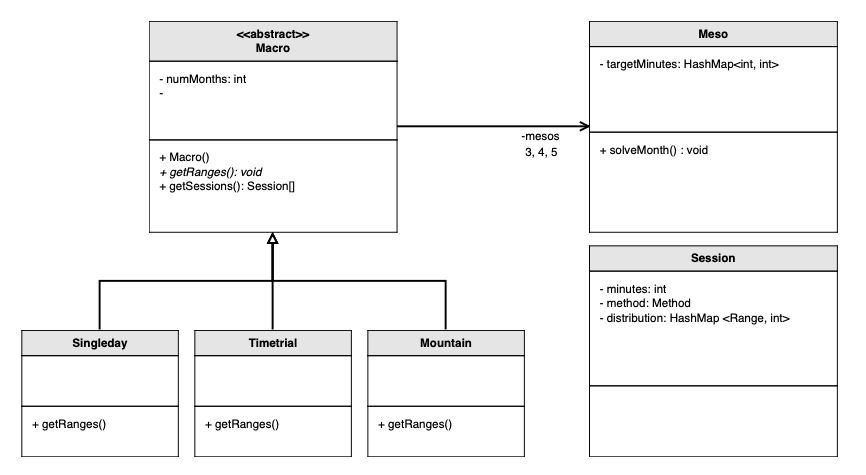
\includegraphics[width=\textwidth]{gfx/SOLVER.png}
% 	\caption{UML Diagramm der  Modellierung}
% 	\label{fig:system:example1}
% \end{figure}
Die Optimierung findet auf Ebene der Mesozyklen statt, sodass auch eine Parallelisierung der ein
\section{Benutzereingaben}
Um den Trainingsplan zu individualisieren erfasst das Programm die Eingaben des Nutzers. \newline
Die Wettkampfart korreliert mit dem Trainingsziel. An der ausgewählten Disziplin richten sich die \newline
Der wöchentliche Trainingsumfang des Plans limitiert die Trainingszeit pro Woche. Die Anzahl der Stunden lässt auch Rückschlüsse auf die Professionalität zu. Während im Profibereich der Trainingsumfang über 20 Stunden beträgt, unterschreiten Amateure diesen Wert üblicherweise. Bei einem Wert um die 5 Stunden, spricht man von Hobbysport. \newline
Nicht nur die wöchentlichen Stunden, sondern auch die wöchentlichen Trainingstage werden bei der Erstellung des Plans berücksichtigt. Die Anzahl der Tage steuert die Häufigkeit der Einheiten.
Wie in \ref{grundlagen:sport:belastungsbereiche} aufgeführt, umfasst ein Training 
 % Weitestgehend entsprechen die Konstanten den Eingaben des Benutzers.
\begin{itemize}
    \item Ziel/Disziplin \cite[S.11]{Radsporttraining} unterschiedlicher Gewichtung\cite[S.14]{Radsporttraining}
    \item wöchentlicher Trainingsumfang: Anzahl Stunden
    \item wöchentliche Trainingstage: Anzahl Tage
    \item Wettkampfstermin: Datum
    \item Dauer des Plans: 3/4/5 Monate
    \begin{itemize}
        \item Straßeneinzelrennen
        \item Rundstrecke
        \item Bergzeitfahrt
    \end{itemize}
\end{itemize}

Einbettung des Solvers in Java Programm
\begin{itemize}
    \item Inhalte der JSON-Objekte (siehe \ref{sec:modellierung:output})
    \item API verfügbar für andere Anwendungen?
    \item Parallelisierung der Mesozyklen. Um Laufzeit zu sparen ist die Optimierung der einzelnen Monate parallelisiert.
    \item Time Limits oder andere Arten zur Steuerung des Solvers -> Kommt dann in Implementierung
\end{itemize}

\begin{figure}[htb]
    \begin{tikzpicture}
        \umlclass[y=5, fill=white]{Macro}{}{}
        \umlclass[x=6, y=5, fill=white]{Meso}{}{}
        \umlclass[x=6, y=0, fill=white]{Session}{}{}
        \umlclass[x=-3, fill=white]{Strasseneinzel}{}{}
        \umlclass[x=0, fill=white]{Rundfahrt}{}{}
        \umlclass[x=3, fill=white]{Bergfahrt}{}{}
        
        \umlVHVinherit[]{Strasseneinzel}{Macro}
        \umlVHVinherit[]{Rundfahrt}{Macro}
        \umlVHVinherit[]{Bergfahrt}{Macro}
        \umlVHVassoc[]{Macro}{Meso}
    \end{tikzpicture}
    \caption{Enumeration um sportartspezifisches zu Kapseln}
    \label{fig:uml:solver}
\end{figure}

\section{Modularisierung}
Die Grundlage dieser Arbeit war eine vorangegangene Bachlorarbeit, die der Laufsport betrifft. Mit Ausblick auf die Erweiterung um das Schwimmtraining, ist durch Kombination dieser Arbeiten vorstellbar zu einem Trainingsplan für Triathleten. 
Aus diesem Grund ist die Arbeit modular gegliedert.
Für viele Sportarten gelten die Trainingsprinzipien der Zyklisierung, Periodisierung, progressive Belastung und Superkompensation. Diese Struktur kann für andere Ausdauersportarten übernommen werden. Um die Trainingsplanerstellung für andere Sportarten zu modellieren, sind folgende Erweiterungen im Code nötig.
Die Definition der Leistungsbereiche ist eine Implementierung des Interfaces. Genauso ist die Liste der Trainingsmethoden der Sportart eine andere. Auch diese ist als Interface definiert. 
\begin{itemize}
    \item Übertragbarkeit auf andere Sportarten? Welche Constraints sind speziell für den Radsport vs. allgemeine Trainingsprinzipien
    \item modulare Entwicklung der Anwendung?
\end{itemize}

\begin{figure}[h]
    \centering
    \begin{tikzpicture}
        \umlclass[type=enumeration, fill=white]{Range}{
            Kompensation   \\ 
            Grundlagenausdauer   \\ 
            Entwicklungsbereich   \\ 
            Spitzenbereich   \\ 
            Kraftausdauer1   \\ 
            Kraftausdauer4   
        }{}
        
        \umlclass[type=enumeration, x=5, fill=white]{Method}{
            Pause \\
            Dauerleistung   \\ 
            Fahrtspiel  \\
            Intervall \\
            Wiederholung  \\
        }{}
        \umlclass[type=enumeration, x=10, fill=white]{SessionName}{
            Pause\\
            Kompensationstraining \\
            ExtensiveFahrt   \\ 
            Fettstoffwechsel  \\
            IntensiveFahrt \\
            ExtensiveKraftausdauerfahrt  \\
            Einzelzeitfahrt  \\
            ExtensivesFahrtspiel  \\
            IntensivesFahrtspiel  \\
            IntensiveKraftausdauer  \\
            Schnelligkeitsausdauer  \\
            Sprinttraining  \\
        }{
            getPause() \\
            getDL() \\
            getFS() \\
            getIV() \\
            getWH() \\
        }
    \end{tikzpicture}    
    \caption{Enumeration um sportartspezifisches zu Kapseln}
    \label{fig:uml:enumeration}
\end{figure}

\section{Ausgabe des Trainingsplans oder Frontend}
Liste von Trainingseinheiten
\label{sec:modellierung:output}
Die Ausgabe des Plans ist eine Liste der Trainingseinheiten. Die Trainingseinheit definiert 
\begin{itemize}
    \item Tag: Datum
    \item Dauer: Anzahl h
    \item Trainingsbereich: \ref{grundlagen:sport:belastungsbereiche}
    \item Trainingsmethode: $\{Pause, Dauerleistung, Intervall, Wiederholung, Fahrtspiel\}$ \ref{grundlagen:methoden}
    \item ? Trainingsalternativen = Auswahl an möglichen Einheiten
\end{itemize}

\begin{itemize}
    \item Darstellung der Trainingseinheiten als Liste in der Java Applikation
    \item Implementierung verfügbar unter \url{http://www.tba.com}
\end{itemize}

\begin{figure}[h]
    \begin{tikzpicture}
        \umlclass[y=5, fill=white]{Main}{}{}
        \umlclass[x=10, y=5, fill=white]{OutputTable}{}{}
        
        \umlVHVassoc[]{Main}{OutputTable}
    \end{tikzpicture}    
    \caption{Enumeration um sportartspezifisches zu Kapseln}
    \label{fig:uml:solver}
\end{figure}

